\documentclass[10pt,a4paper, margin=1in]{article}
\usepackage{fullpage}
\usepackage{amsfonts, amsmath, pifont}
\usepackage{amsthm}
\usepackage{graphicx}
\usepackage{pgfplots}
\usepackage{tikz}
\usepackage{float}
\usepackage{tkz-euclide}
\usepackage{steinmetz}
\pgfplotsset{compat=1.13}

\usetikzlibrary{angles,quotes}


\begin{filecontents}{q1a.dat}
 n   xn
 -4   0
 -3   0
 -2   0
 -1  0.5
 0   0.5
 1   0.5
 2   0
 3   0
 4   0 
\end{filecontents}

\begin{filecontents}{q1b_1.dat}
 n   xn
 -4   0
 -3   0
 -2   0
 -1  1
 0   1.5
 1   1
 2   0
 3   0
 4   0 
\end{filecontents}

\begin{filecontents}{q1b_2.dat}
 n   xn
 -4   0
 -3   0
 -2   0
 -1  1
 0   0
 1   -1
 2   0
 3   0
 4   0 
\end{filecontents}

\begin{filecontents}{q1c_1.dat}
 n   xn
 -4   0
 -3   0
 -2   0.5
 -1  1.11
 0   2
 1   1.11
 2   0.5
 3   0
 4   0 
\end{filecontents}

\begin{filecontents}{q1c_2.dat}
 n   xn
 -4   0
 -3   0
 -2   -1
 -1  2
 0   0
 1   -2
 2   1
 3   0
 4   0 
\end{filecontents}

\begin{filecontents}{q2.dat}
 n   xn
 -3   0.33
 -2   0.5
 -1  0.25
 0   1
 1   0.25
 2   0.5
 3   0.33
\end{filecontents}

\begin{filecontents}{q7a.dat}
 n   xn
-4    1
-3    -0.5
-2    0
-1    -0.5
0    1
1    -0.5
2    0
3    -0.5
4	 1
5    -0.5
6    0
7    -0.5
\end{filecontents}


\begin{filecontents}{q7b_1.dat}
 n   xn
-4   3
-3   2
-2   1
-1   2
0    3
1    2
2    1
3    2
4	 3
5    2
6    1
7    2
\end{filecontents}

\begin{filecontents}{q7b_2.dat}
 n   xn
-4   0
-3   -1
-2   0
-1   1
0    0
1    -1
2    0
3    1
4	 0
5    -1
6    0
7    1
\end{filecontents}

\usepackage{geometry}
 \geometry{
 a4paper,
 total={210mm,297mm},
 left=10mm,
 right=10mm,
 top=10mm,
 bottom=10mm,
 }
 % Write both of your names here. Fill exxxxxxx with your ceng mail address.
 \author{
  BAŞŞİMŞEK, Orçun\\
  \texttt{e2098804@ceng.metu.edu.tr}
  \and
  TONKAL, Özlem\\
  \texttt{e1881531@ceng.metu.edu.tr}
}
\title{CENG 384 - Signals and Systems for Computer Engineers \\
Spring 2021 \\
Homework 3}
\begin{document}
\maketitle



\noindent\rule{19cm}{1.2pt}

\begin{enumerate}

\item %write the solution of q1
    \begin{enumerate}
    % Write your solutions in the following items.
    \item %write the solution of q1a
    \[ x(t) = \frac{1}{2} + \cos(w_ot) \]
    \[ = \frac{1}{2} + \frac{1}{2}(e^{jw_ot} + e^{-jw_ot}) \]
    \[ = \frac{1}{2} + \frac{1}{2}e^{jw_ot} + \frac{1}{2}e^{-jw_ot} \]
    Therefore, $a_0 = \frac{1}{2}$ \ ,\ $a_1 = \frac{1}{2}$ \ and \ $a_{-1} = \frac{1}{2}$. Magnitude graph is:
    
    \begin{figure} [H]
    \centering
    \begin{tikzpicture}[scale=0.6] 
      \begin{axis}[
          axis lines=middle,
          xlabel={$k$},
          ylabel={$\boldsymbol{|a_k|}$},
          xtick={-4, -3, -2, -1, 0, 1,2,3,4},
          ytick={0, 0.5, 1},
          ymin=0, ymax=1,
          xmin=-4, xmax=4,
          every axis x label/.style={at={(ticklabel* cs:1.05)}, anchor=west,},
          every axis y label/.style={at={(ticklabel* cs:1.05)}, anchor=south,},
          grid,
        ]
        \addplot [ycomb, black, thick, mark=*] table [x={n}, y={xn}] {q1a.dat};
      \end{axis}
    \end{tikzpicture}
    \caption{$k$ vs. $|a_k|$}
    \label{fig:q1a}
\end{figure}

All phases are $0$. Therefore, phase graph is not drawn.

    \item %write the solution of q1b
    \[ y(t) = \frac{3}{2} + 2\sin(w_ot) \]
    \[ = \frac{3}{2} + 2[\frac{1}{2j}(e^{jw_ot} - e^{-jw_ot})] \]
      \[ = \frac{3}{2} + \frac{1}{j}e^{jw_ot} - \frac{1}{j}e^{-jw_ot} \]
      Therefore, $b_0 = \frac{3}{2}$ \ ,\ $b_1 = \frac{1}{j}$ \ and \ $b_{-1} = - \frac{1}{j}$. Magnitude graph is:
      
      \begin{figure} [H]
    \centering
    \begin{tikzpicture}[scale=0.6] 
      \begin{axis}[
          axis lines=middle,
          xlabel={$k$},
          ylabel={$\boldsymbol{|b_k|}$},
          xtick={-4, -3, -2, -1, 0, 1,2,3,4},
          ytick={0, 0.5, 1, 1.5},
          ymin=0, ymax=2,
          xmin=-4, xmax=4,
          every axis x label/.style={at={(ticklabel* cs:1.05)}, anchor=west,},
          every axis y label/.style={at={(ticklabel* cs:1.05)}, anchor=south,},
          grid,
        ]
        \addplot [ycomb, black, thick, mark=*] table [x={n}, y={xn}] {q1b_1.dat};
      \end{axis}
    \end{tikzpicture}
    \caption{$k$ vs. $|b_k|$}
    \label{fig:q1b_1}
\end{figure}

Phase graph is: 

\begin{figure} [H]
    \centering
    \begin{tikzpicture}[scale=0.8] 
      \begin{axis}[
          axis lines=middle,
          xlabel={$k$},
          ylabel={$\boldsymbol{\phase{b_k}}$},
          xtick={-4, -3, -2, -1, 0, 1,2,3,4},
          ytick={-1, 0, 1},
          yticklabels={$- \frac{\pi}{2}$, 0,$ \frac{\pi}{2}$},
          ymin=-2, ymax=1,
          xmin=-4, xmax=4,
          every axis x label/.style={at={(ticklabel* cs:1.05)}, anchor=west,},
          every axis y label/.style={at={(ticklabel* cs:1.05)}, anchor=south,},
          grid,
        ]
        \addplot [ycomb, black, thick, mark=*] table [x={n}, y={xn}] {q1b_2.dat};
      \end{axis}
    \end{tikzpicture}
    \caption{$k$ vs. $\phase{b_k}$}
    \label{fig:q1b_2}
\end{figure}
    \item %write the solution of q1c
    \[ z(t) = x(t) + y(t) =  \frac{1}{2} + \cos(w_ot) +  \frac{3}{2} + 2\sin(w_ot) + \cos(2w_ot + \frac{\pi}{4}) \]
    \[ =  \frac{1}{2} + \frac{1}{2}(e^{jw_ot} + e^{-jw_ot}) +  \frac{3}{2} + 2[\frac{1}{2j}(e^{jw_ot} - e^{-jw_ot})] + \frac{1}{2}(e^{j(2w_ot + \frac{\pi}{4})} + e^{-j(2w_ot + \frac{\pi}{4})}) \]
     \[ =  \frac{1}{2} + (\frac{1}{2} + \frac{1}{j})e^{jw_ot} + \frac{3}{2} + (\frac{1}{2} - \frac{1}{j})e^{-jw_ot}  + (\frac{e^{j \pi/4}}{2})e^{j2w_ot} + (\frac{e^{-j \pi/4}}{2})e^{-j2w_ot} \]
     \[ =  2 + (\frac{j+2}{2j})e^{jw_ot} +  (\frac{j-2}{2j})e^{-jw_ot}  + (\frac{e^{j \pi/4}}{2})e^{j2w_ot} + (\frac{e^{-j \pi/4}}{2})e^{-j2w_ot} \]
     Therefore, Fourier coefficients are:
     \[ c_0 = 2 \]
     \[ c_1 = \frac{j+2}{2j} = \frac{1}{2} - j \]
     \[ c_{-1} = \frac{j-2}{2j} = \frac{1}{2} + j \]
     \[ c_2 = \frac{e^{j \pi/4}}{2} = \frac{\sqrt{2}}{4}(1+j) \]
     \[ c_{-2} = \frac{e^{-j \pi/4}}{2} = \frac{\sqrt{2}}{4}(1-j) \]
     Magnitude graph is: 
     
     \begin{figure} [H]
    \centering
    \begin{tikzpicture}[scale=0.8] 
      \begin{axis}[
          axis lines=middle,
          xlabel={$k$},
          ylabel={$\boldsymbol{|c_k|}$},
          xtick={-4, -3, -2, -1, 0, 1,2,3,4},
          ytick={0, 0.5, 1.11, 2},
          ymin=0, ymax=3,
          xmin=-4, xmax=4,
          every axis x label/.style={at={(ticklabel* cs:1.05)}, anchor=west,},
          every axis y label/.style={at={(ticklabel* cs:1.05)}, anchor=south,},
          grid,
        ]
        \addplot [ycomb, black, thick, mark=*] table [x={n}, y={xn}] {q1c_1.dat};
      \end{axis}
    \end{tikzpicture}
    \caption{$k$ vs. $|c_k|$}
    \label{fig:q1c_1}
\end{figure}

Phase graph is: 

\begin{figure} [H]
    \centering
    \begin{tikzpicture}[scale=0.8] 
      \begin{axis}[
          axis lines=middle,
          xlabel={$k$},
          ylabel={$\boldsymbol{\phase{c_k}}$},
          xtick={-4, -3, -2, -1, 0, 1,2,3,4},
          ytick={-2, -1, 0, 1, 2},
          yticklabels={$- 0.35\pi $, $-\frac{\pi}{4} $, 0, $\frac{\pi}{4}$, $ 0.35\pi $},
          ymin=-3, ymax=3,
          xmin=-4, xmax=4,
          every axis x label/.style={at={(ticklabel* cs:1.05)}, anchor=west,},
          every axis y label/.style={at={(ticklabel* cs:1.05)}, anchor=south,},
          grid,
        ]
        \addplot [ycomb, black, thick, mark=*] table [x={n}, y={xn}] {q1c_2.dat};
      \end{axis}
    \end{tikzpicture}
    \caption{$k$ vs. $\phase{c_k}$}
    \label{fig:q1c_2}
\end{figure}
    \end{enumerate}

\item %write the solution of q2

\[x(t) = \begin{cases}
	  M & t < T_1 \\ 
	  0 & T_1\leq t < T \\

   \end{cases}
\]
\\
\[a_0 = \begin{cases}
	   \frac{1}{T} * \int_{0}^{T_1} x(t) \,dt\  & t < T_1 \\ 
	   \frac{1}{T} * \int_{0}^{T_1} x(t) \,dt\  & T_1\leq t < T \\

   \end{cases}
\]
\\
\[a_0 = \begin{cases}
	  \frac{1}{T} * \int_{0}^{T_1} M \,dt\  & t < T_1 \\ 
	  \frac{1}{T} * \int_{0}^{T_1} 0 \,dt\  & T_1\leq t < T \\

   \end{cases}
\]
\\
\[a_0 = \begin{cases}
	  \frac{1}{T} * (M*T_1 - 0 )  & t < T_1 \\ 
	  \frac{1}{T} * 0  & T_1\leq t < T \\

   \end{cases}
\]
\\
\[a_0 = \begin{cases}
	  \frac{M*T_1}{T}  & t < T_1 \\ 
         0   & T_1\leq t < T \\

   \end{cases}
\]
\\
$A_0 = 2 * a_0$
\\
\[A_0 = \begin{cases}
	  2*\frac{M*T_1}{T}  & t < T_1 \\ 
         0   & T_1\leq t < T \\

   \end{cases}
\]
\\
\\
$b_0 = \frac{2}{T} * \int_{0}^{T_1} x(t)*cos(k W_0 t) \,dt\ $
\\
\[b_0 = \begin{cases}
	   \frac{2}{T} * \int_{0}^{T_1} M*cos(k W_0 t) \,dt\  & t < T_1 \\ 
	   \frac{2}{T} * \int_{0}^{T_1} 0*cos(k W_0 t) \,dt\  & T_1\leq t < T \\

   \end{cases}
\]
\\
\[b_0 = \begin{cases}
	   \frac{2*M}{T*k*W_0} * ( sin(k W_0 T1) - 0 )  & t < T_1 \\ 
	   0  & T_1\leq t < T \\

   \end{cases}
\]
\\
$A_k = b_0$
\\
\[A_k = \begin{cases}
	   \frac{2*M}{T*k*W_0} * ( sin(k W_0 T1) - 0 )  & t < T_1 \\ 
	   0  & T_1\leq t < T \\

   \end{cases}
\]
\\

$c_0 = \frac{2}{T} * \int_{0}^{T_1} x(t)*sin(k W_0 t) \,dt\ $
\\
\[c_0 = \begin{cases}
	   \frac{2}{T} * \int_{0}^{T_1} M*sin(k W_0 t) \,dt\  & t < T_1 \\ 
	   \frac{2}{T} * \int_{0}^{T_1} 0*sin(k W_0 t) \,dt\  & T_1\leq t < T \\

   \end{cases}
\]
\\
\[c_0 = \begin{cases}
	   \frac{-2*M}{T*k*W_0} * ( cos(k W_0 T1) - 1 )  & t < T_1 \\ 
	   0  & T_1\leq t < T \\

   \end{cases}
\]
\\
$_k = - c_0$
\\
\[B_0 = \begin{cases}
	   \frac{2*M}{T*k*W_0} * ( cos(k W_0 T1) - 1 )  & t < T_1 \\ 
	   0  & T_1\leq t < T \\

   \end{cases}
\]
\\
     Magnitude graph is: 

    \begin{figure} [H]
    \centering
    \begin{tikzpicture}[scale=0.6] 
      \begin{axis}[
          axis lines=middle,
          xlabel={$k$},
          ylabel={$\boldsymbol{|a_k|}$},
          xtick={-4, -3, -2, -1, 0, 1,2,3,4},
          ytick={0, 0.33,0.25, 0.5,1},
          ymin=0, ymax=1,
          xmin=-4, xmax=4,
          every axis x label/.style={at={(ticklabel* cs:1.05)}, anchor=west,},
          every axis y label/.style={at={(ticklabel* cs:1.05)}, anchor=south,},
          grid,
        ]
        \addplot [ycomb, black, thick, mark=*] table [x={n}, y={xn}] {q2.dat};
      \end{axis}
    \end{tikzpicture}
    \caption{$k$ vs. $|a_k|$}
    \label{fig:q1a}
\end{figure}


\item %write the solution of q3  
    \begin{enumerate}
    % Write your solutions in the following items.
    \item %write the solution of q3a

    x(t) = 1+ $ \frac{1}{2}*cos(2 \pi t)  + cos(4 \pi t) +  \frac{2}{3}* cos(6 \pi t) $
    
    \begin{figure} [H]
        \centering

            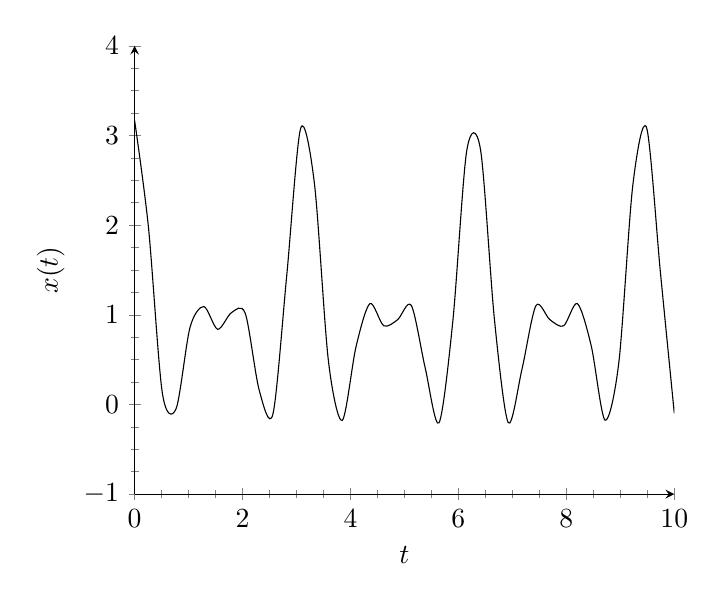
\begin{tikzpicture}
            %\color{white}
            \begin{axis}[
              minor tick num=3,
              axis y line=left,
              axis x line=bottom,
              xlabel=$t$,ylabel=$x(t)$,
            %  yticklabels=\empty,
              ymax=4,
              ymin=-1,
              background/.style={fill=gray},
            ]
            \addplot[smooth,black,mark=none, domain=0:10,samples=40]
            {1+ (1/2)* cos(deg(2*x)) + cos(deg(4*x)) + (2/3) * cos(deg(6*x)) };
            \end{axis}
            \end{tikzpicture}

        \caption{$x(t)$ vs $t$.}
        \label{fig:3a}
    \end{figure}
    
    
    
    \item %write the solution of q3b

    
    x(t) = 1+ $ \frac{1}{2}*cos(2 \pi t)  + cos(4 \pi t) +  \frac{2}{3}* cos(6 \pi t) $
    \\
    $x(t) = \frac{1}{2}*(\frac{1}{2}*(e^{j 2 \pi t} + e^{-j 2 \pi t}) + \frac{1}{2}*(e^{2 j 2 \pi t} + e^{- 2 j 2 \pi t}) + (\frac{2}{3} *( \frac{1}{2}*(e^{3 j 2 \pi t} + e^{- 3 j 2 \pi t}))  $
    \\
    $x(t) = \frac{1}{4}*(e^{j 2 \pi t} + e^{-j 2 \pi t}) + \frac{1}{2}*(e^{2 j 2 \pi t} + e^{- 2 j 2 \pi t}) +  \frac{1}{3}*(e^{3 j 2 \pi t} + e^{- 3 j 2 \pi t})  $
    \\
    \\
    $a_0=1
    \\
    a_1=a_{-1 = \frac{1}{4}}
    \\
    a_2=a_{-2}=\frac{1}{2}
    \\a_3=a_{-3}=\frac{1}{3}$
    
    \item %write the solution of q3c
    
    In $a_k$ graph we use frequency domain which is how much of signal exist within a given frequency.
    In $x_t$ graph we see signal behavior in given time domain.Signal properties are same but we observe them different way.
    \\
    
    \item %write the solution of q3d
    
        $b_k = a_k * H(j k W_0)
    \\
    H(j W_0) = \int_{-\infty}^{\infty} h(t)e^{-j w_0 t} \,dt\
    \\
    H(j W_0) = \int_{-\infty}^{\infty} e^{-2 t}u(t) e^{-j w_0 t} \,dt\
    \\
     H(j W_0) = \int_{0}^{\infty} e^{-2 t} e^{-j w_0 t} \,dt\
     \\
     H(j W_0) = \frac{1}{2+j W_0}
     \\
     H(j k W_0) = \frac{1}{2+j k W_0}\\
    $
    \\
    Fundamental period T is 1. Fundamental frequency $ W_0$ is $\frac{2\pi}{T} = 2 \pi$
    \\
    $b_k = a_k * \frac{1}{2 + j k 2 \pi}
    \\
    b_0 = 1 * \frac{1}{2-0} =  \frac{1}{2} 
    \\
    b_1 = \frac{1}{4} * \frac{1}{2 + j 2 \pi} =  \frac{1}{8*(1 + \pi j)}
    \\
    b_{-1} = \frac{1}{4} * \frac{1}{2 - j 2 \pi} =  \frac{1}{8*(1 - \pi j)}
    \\
    b_2 = \frac{1}{2} * \frac{1}{2 + j 4 \pi} =  \frac{1}{4*(1 + 2 \pi j)}
    \\
    b_{-2} = \frac{1}{2} * \frac{1}{2 - j 4 \pi} =  \frac{1}{4*(1 - 2 \pi j)}
    \\
    b_3 = \frac{1}{3} * \frac{1}{2 + j 6 \pi} =  \frac{1}{6*(1 + 3 \pi j)}
    \\
    b_{-3} = \frac{1}{3} * \frac{1}{2 - j 6 \pi} =  \frac{1}{6*(1 - 3 \pi j)}    
    $
    \end{enumerate}

\item %write the solution of q4
    \begin{enumerate}
    % Write your solutions in the following items.
    
        
    \item %write the solution of q4a
    Basic periodic signal is x(t) = $e^{j W_0 t}$
    \\
    $a_k = \frac{1}{4} \int_{T}^{} x(t ) e^{-j k  w_0 t} \,dt\ $
        $x(t) => a_k
    \\
    x(t-3) => b_k$
    \\ 
    Because of time shifting;
    $b_k = e^{-j k W_0 3}*a_k $
    \\
    $x(-t) => b_k$
    \\ 
    Because of time reversal;
    $b_k = a_{-k} $
    \\
    Because of linearity ;
    $\frac{e^{-j k W_0 3}*a_k }{3} - \frac{2}{7} * a_k $
    \item %write the solution of q4b
    
        $f'(x) = c_k $
    \\
    Because of differentiation property;
    $c_k = j W_0 k * a_k$
    \\
    $(f'(x))^3 = d_x 
    \\
    d_x = j^3 (W_0)^3 a_k $
    \end{enumerate}

\item %write the solution of q5
    \begin{enumerate}
    % Write your solutions in the following items.
    \item %write the solution of q5a
    $x[n] = \sin(\frac{\pi}{2}n)$ \ \ it is periodic with fundamental period: $N = \frac{2\pi}{\frac{\pi}{2}} = 4$ \\
    $x[n] = \frac{1}{2j}(e^{j\frac{\pi}{2}n} - e^{-j\frac{\pi}{2}n})$ \\
    Therefore, Fourier coefficients of $x[n]$ are: \\
    $a_1 = \frac{1}{2j}$ \ and \ $a_{-1} = -\frac{1}{2j}$ \\
    \item %write the solution of q5b
    $y[n] = 1+ \cos(\frac{\pi}{2}n)$ \ \ it is periodic with fundamental period: $N = \frac{2\pi}{\frac{\pi}{2}} = 4$ \\
    $y[n] = 1+ \frac{1}{2}(e^{j\frac{\pi}{2}n} + e^{-j\frac{\pi}{2}n})$ \\
    Therefore, Fourier coefficients of $y[n]$ are: \\
    $b_0 = 1$ \ , \ $b_1 = \frac{1}{2}$ \ and \ $b_{-1} =\frac{1}{2}$ \\
    
    \item %write the solution of q5c
    According to multiplication property, since our signals are periodic with same period $T = 4$, fourier series coefficients of their multiplication $x[n] \times y[n]$ will be : \\
    \[ h_k = \sum_{l=-\infty}^{\infty} a_lb_{k-l} \]
    We can use convolution for the right hand side of this equation like $h_k = a_k * b_k$. Therefore: \\
    $a_k = \frac{1}{2j} \delta[k-1] - \frac{1}{2j} \delta[k+1] $  \ from part a \\
     $b_k = \delta[k] + \frac{1}{2} \delta[k-1] + \frac{1}{2} \delta[k+1] $  \ from part a \\
     \[ h_k = (\frac{1}{2j} \delta[k-1] - \frac{1}{2j} \delta[k+1]) * (\delta[k] + \frac{1}{2} \delta[k-1] + \frac{1}{2} \delta[k+1]) \]
     \[ = \frac{1}{2j} \delta[k-1] + \frac{1}{4j} \delta[k-2] + \frac{1}{4j} \delta[k] - \frac{1}{2j} \delta[k+1] - \frac{1}{4j} \delta[k] - \frac{1}{4j} \delta[k+2] \]
     \[h_k = \frac{1}{2j} \delta[k-1] + \frac{1}{4j} \delta[k-2] - \frac{1}{2j} \delta[k+1] - \frac{1}{4j} \delta[k+2] \] \\
     Therefore: $h_1 = \frac{1}{2j}$ \ , \ $h_2 = \frac{1}{4j}$ \ , \ $h_{-1} = - \frac{1}{2j}$ \ , \ $h_{-2} = - \frac{1}{4j}$
         
    \item %write the solution of q5d
    \[ x[n] \times y[n] = \sin(\frac{\pi}{2}n) \times (1+ \cos(\frac{\pi}{2}n)) \]
    \[ = \sin(\frac{\pi}{2}n) + (\sin(\frac{\pi}{2}n) \times \cos(\frac{\pi}{2}n)) \]
    \[ = \sin(\frac{\pi}{2}n) + \frac{1}{2}(\sin(\frac{\pi}{2}n + \frac{\pi}{2}n) + \sin(\frac{\pi}{2}n - \frac{\pi}{2}n)) \]
     \[ = \sin(\frac{\pi}{2}n) + \frac{1}{2}(\sin(\pi n) + 0) \]
        \[ = \sin(\frac{\pi}{2}n) + \frac{1}{2}\sin(\pi n) \]
        \[ = \frac{1}{2j}e^{j\frac{\pi}{2}n} - \frac{1}{2j}e^{-j\frac{\pi}{2}n} + \frac{1}{2}\sin(\pi n) \]
        \[ = \frac{1}{2j}e^{j\frac{\pi}{2}n} - \frac{1}{2j}e^{-j\frac{\pi}{2}n} + \frac{1}{2}(\frac{1}{2j}e^{j \pi n} - \frac{1}{2j}e^{-j \pi n})  \]
        \[ = \frac{1}{2j}e^{j\frac{\pi}{2}n} - \frac{1}{2j}e^{-j\frac{\pi}{2}n} + \frac{1}{4j}e^{2j \frac{\pi}{2} n} - \frac{1}{4j}e^{-2j \frac{\pi}{2} n}  \]
        Therefore, $h_1 = \frac{1}{2j}$ \ , \ $h_2 = \frac{1}{4j}$ \ , \ $h_{-1} = - \frac{1}{2j}$ \ , \ $h_{-2} = - \frac{1}{4j}$ \\
        We got the same result that we have already found in part c.
    \end{enumerate}

\item %write the solution of q6
\[ a_k = \cos(\frac{k\pi}{6}) + \sin(\frac{5k\pi}{6}) \]
\[ a_k = \frac{1}{2}(e^{jk\frac{\pi}{6}} + e^{-jk\frac{\pi}{6}}) + \frac{1}{2j}(e^{j5k\frac{\pi}{6}} - e^{-j5k\frac{\pi}{6}}) \]
\[ a_k = \frac{1}{2}e^{j\frac{\pi}{6}k} + \frac{1}{2}e^{-j\frac{\pi}{6}k} + \frac{1}{2j}e^{j\frac{5\pi}{6}k} -\frac{1}{2j}e^{-j\frac{5\pi}{6}k} \]

We know $N = 12$. By considering analysis equation $a_k = \frac{1}{N} \sum_{n=N}^{} x[n]e^{-jk(2\pi/N)n}$, we can create below similarity easily: \\
\[ a_k = \frac{1}{2}e^{j\frac{2\pi}{12}k1} + \frac{1}{2}e^{-j\frac{2\pi}{12}k1} + \frac{1}{2j}e^{j\frac{2\pi}{12}k5} -\frac{1}{2j}e^{-j\frac{2\pi}{12}k5} \]
However, we need to $e^{-j}$ at each term to create a full similarity to the analysis equation. For this reason, we can use $e^{-j2\pi k}$ which is actually equals to $1$ according to Euler equation: \\
$e^{-j2\pi k} = \cos(-2\pi k) + j\sin(-2\pi k) = \cos(-2\pi k) = 1$ \\
By multiplying the terms that do not contain $e^{-j}$ in our equation with $e^{-j2\pi k}$, we get: 
\[ a_k = \frac{1}{2}(e^{-j2\pi k})e^{j\frac{2\pi}{12}k1} + \frac{1}{2}e^{-j\frac{2\pi}{12}k1} + \frac{1}{2j}(e^{-j2\pi k})e^{j\frac{2\pi}{12}k5} -\frac{1}{2j}e^{-j\frac{2\pi}{12}k5} \]
\[ a_k = \frac{1}{2}e^{(-j2\pi k)(1 - \frac{1}{12})} + \frac{1}{2}e^{-j\frac{2\pi}{12}k1} + \frac{1}{2j}e^{(-j2\pi k)(1 - \frac{5}{12})} -\frac{1}{2j}e^{-j\frac{2\pi}{12}k5} \]
\[ a_k = \frac{1}{2}e^{(-j2\pi k)(\frac{11}{12})} + \frac{1}{2}e^{-j\frac{2\pi}{12}k1} + \frac{1}{2j}e^{(-j2\pi k)(\frac{7}{12})} -\frac{1}{2j}e^{-j\frac{2\pi}{12}k5} \]
\[ a_k = \frac{1}{2}e^{-j\frac{2\pi}{12} k \cdot 11} + \frac{1}{2}e^{-j\frac{2\pi}{12}k \cdot 1} + \frac{1}{2j}e^{-j\frac{2\pi}{12} k \cdot 7} -\frac{1}{2j}e^{-j\frac{2\pi}{12}k \cdot 5} \ (eq. \ 1) \]

Now, we can use analysis equation without any problem. We also already know $N=12$. Therefore:
\[ a_k = \frac{1}{N} \sum_{n=N}^{} x[n]e^{-jk(2\pi/N)n} \]
\[ a_k = \frac{1}{12} \sum_{n=0}^{11} x[n]e^{-jk(2\pi/12)n} \]
\[ a_k = \frac{1}{12} (x[0]e^{-jk(2\pi/12) \cdot 0} + x[1]e^{-jk(2\pi/12) \cdot 1} + x[2]e^{-jk(2\pi/12) \cdot 2} + \ ... \ + x[11]e^{-jk(2\pi/12) \cdot 11}) \]

Here, we can easily say that we have nonzero Fourier coefficients for only $n =  1, 5, 7, 11$ by checking our derived equation above (eq .1).
\[ for \ n=1: \ \frac{1}{12} x[1] = \frac{1}{2} , \ so \ x[1] = 6 \]
\[ for \ n=5: \ \frac{1}{12} x[5] = - \frac{1}{2j} , \ so \ x[5] = 6j \]
\[ for \ n=7: \ \frac{1}{12} x[7] = \frac{1}{2j} , \ so \ x[7] = -6j \]
\[ for \ n=11: \ \frac{1}{12} x[11] = \frac{1}{2} , \ so \ x[11] = 6 \]
Therefore, according to these values, our signal $x[n]$ will be:
\[ x[n] = 6\delta[n-1] + 6j\delta[n-5] - 6j\delta[n-7] + 6\delta[n-11] \]

\item %write the solution of q7
    \begin{enumerate}
    % Write your solutions in the following items.
    \item %write the solution of q7a
    $N = 4$ \\
    We can use analysis equation. It is: \\
    \[ a_k = \frac{1}{N} \sum_{n=N}^{} x[n]e^{-jk(2\pi/N)n} \]
    \[ = \frac{1}{4} \sum_{n=0}^{3} x[n]e^{-jk(2\pi/4)n} \]
    \[ = \frac{1}{4}(x[0] + x[1]e^{-jk(2\pi/4)} + x[2]e^{-jk(2\pi/4)2} + x[3]e^{-jk(2\pi/4)3}) \]
     \[ = \frac{1}{4}(0 + e^{-jk(2\pi/4)} + 2e^{-jk(2\pi/4)2} + e^{-jk(2\pi/4)3}) \]
     \[ = \frac{1}{4}(e^{-jk \pi/2} + 2e^{-jk\pi} + e^{-jk3\pi/2}) \]
     \[ = \frac{1}{4}((\cos(-\pi/2) + j\sin(-\pi/2))^k + 2(\cos(-\pi) + j\sin(-\pi))^k + (\cos(-3\pi/2) + j\sin(-3\pi/2) )^k \]
     \[ a_k = \frac{1}{4}((-j)^k + 2(-1)^k + (j)^k) \]
     
     We know that $a_k = a_k + N$ since the signal is periodic with $N = 4$. Therefore, \\
     \[ a_0 = \frac{1}{4}((-j)^0 + 2(-1)^0 + (j)^0) = 1  \]
     \[ a_1 = \frac{1}{4}((-j)^1 + 2(-1)^1 + (j)^1) = \frac{1}{4}(-j - 2 + j) = -\frac{1}{2}  \]
     \[ a_2 = \frac{1}{4}((-j)^2 + 2(-1)^2 + (j)^2) = \frac{1}{4}(-1 + 2 -1) = 0  \]
     \[ a_3 = \frac{1}{4}((-j)^3 + 2(-1)^3 + (j)^3) = \frac{1}{4}(j - 2 -j) = - \frac{1}{2}  \]
     We do not need to find other coefficients, we can just use the period ($N=4$) for other coefficients according to above fact ($a_k = a_k + 4$). Therefore, magnitude graph of $a_k$'s is:
     
        \begin{figure} [H]
    \centering
    \begin{tikzpicture}[scale=1] 
      \begin{axis}[
          axis lines=middle,
          xlabel={$k$},
          ylabel={$\boldsymbol{a_k}$},
          xtick={ -4,-3,-2,-1, 0, 1, 2, 3,4,5,6,7},
          ytick={-1, -0.5, 0, 0.5, 1},
          ymin=-1, ymax=1,
          xmin=-4, xmax=7,
          every axis x label/.style={at={(ticklabel* cs:1.05)}, anchor=west,},
          every axis y label/.style={at={(ticklabel* cs:1.05)}, anchor=south,},
          grid,
        ]
        \addplot [ycomb, black, thick, mark=*] table [x={n}, y={xn}] {q7a.dat};
      \end{axis}
    \end{tikzpicture}
    \caption{$k$ vs. $a_k$ (continues towards left and right with period N=4)}
    \label{fig:q7a}
\end{figure}

Also, it is easily seen that spectrum graph consists of all $0$. Therefore, it is not drawn.

    \item %write the solution of q7b
    
    \textbf{i.} \ It is easily seen that $y[n]$ is 0 for $n = ..., -5 ,-1 ,3, 7, ...$. However, $x[n]$ is 1 for same $n$ values. This is the only difference between two graphs. Therefore, we can substract 1 from $x[n]$ for these $n$ values to reach $y[n]$ signal. We can use unit impulse for this substraction. \\
    \[ y[n] = x[n] - \sum_{m= -\infty}^{\infty} \delta[n-4m+1] \]
    \textbf{ii.} \\
    $N = 4$ again. \\
    We can use analysis equation. It is: \\
    \[ b_k = \frac{1}{N} \sum_{n=N}^{} y[n]e^{-jk(2\pi/N)n} \]
    \[ = \frac{1}{4} \sum_{n=0}^{3} y[n]e^{-jk(2\pi/4)n} \]
    \[ = \frac{1}{4}(y[0] + y[1]e^{-jk(2\pi/4)} + y[2]e^{-jk(2\pi/4)2} + y[3]e^{-jk(2\pi/4)3}) \]
     \[ = \frac{1}{4}(0 + e^{-jk(2\pi/4)} + 2e^{-jk(2\pi/4)2} \]
     \[ = \frac{1}{4}(e^{-jk \pi/2} + 2e^{-jk\pi}) \]
     \[ = \frac{1}{4}((\cos(-\pi/2) + j\sin(-\pi/2))^k + 2(\cos(-\pi) + j\sin(-\pi))^k \]
     \[ b_k = \frac{1}{4}((-j)^k + 2(-1)^k) \]
     
     We know that $b_k = b_k + N$ since the signal is periodic with $N = 4$. Therefore, \\
     \[ b_0 = \frac{1}{4}((-j)^0 + 2(-1)^0) = \frac{3}{4}  \]
     \[ b_1 = \frac{1}{4}((-j)^1 + 2(-1)^1) = \frac{-j-2}{4} \]
     \[ b_2 = \frac{1}{4}((-j)^2 + 2(-1)^2) = \frac{1}{4}(-1 + 2) = \frac{1}{4}  \]
     \[ b_3 = \frac{1}{4}((-j)^3 + 2(-1)^3) = \frac{1}{4}(j - 2) =  \frac{j-2}{4}  \]
     We do not need to find other coefficients, we can just use the period ($N=4$) for other coefficients according to above fact ($b_k = b_k + 4$). Magnitudes are: \\
     
     \[ |b_0| = \sqrt{(\frac{3}{4})^2 + 0^2} = \frac{3}{4} \]
     \[ |b_1| = \sqrt{(\frac{-2}{4})^2 + (\frac{-1}{4})^2} = \sqrt{\frac{5}{16}} \]
     \[ |b_2| = \sqrt{(\frac{1}{4})^2 + 0^2} = \frac{1}{4} \]
     \[ |b_3| = \sqrt{(\frac{-2}{4})^2 + (\frac{1}{4})^2} = \sqrt{\frac{5}{16}} \]
     
     
     Therefore, magnitude graph of $b_k$'s is:
     \begin{figure} [H]
    \centering
    \begin{tikzpicture}[scale=1] 
      \begin{axis}[
          axis lines=middle,
          xlabel={$k$},
          ylabel={$\boldsymbol{|b_k|}$},
          xtick={ -4,-3,-2,-1, 0, 1, 2, 3,4,5,6,7},
          ytick={0,1,2,3},
          yticklabels={0, $\frac{1}{4}$, $\sqrt{\frac{5}{16}}$, $\frac{3}{4}$},
          ymin=0, ymax=3,
          xmin=-4, xmax=7,
          every axis x label/.style={at={(ticklabel* cs:1.05)}, anchor=west,},
          every axis y label/.style={at={(ticklabel* cs:1.05)}, anchor=south,},
          grid,
        ]
        \addplot [ycomb, black, thick, mark=*] table [x={n}, y={xn}] {q7b_1.dat};
      \end{axis}
    \end{tikzpicture}
    \caption{$k$ vs. $|b_k|$ (continues towards left and right with period N=4)}
    \label{fig:q7b_1}
\end{figure}

Phases are: \\
\[ \phase{b_0} = \arctan(0) = 0 \]
\[ \phase{b_1} = \arctan(\frac{-\frac{1}{4}}{-\frac{2}{4}}) - \pi (since \ it \ is \ in \ third \ region \ in \ unit \ circle)  = -0.85\pi \]
\[ \phase{b_2} = \arctan(0) = 0 \]
\[ \phase{b_3} = \arctan(\frac{\frac{1}{4}}{-\frac{2}{4}}) + \pi (since \ it \ is \ in \ second \ region \ in \ unit \ circle)  = 0.85\pi \]

The phase graph of $b_k$'s is: \\
 \begin{figure} [H]
    \centering
    \begin{tikzpicture}[scale=1] 
      \begin{axis}[
          axis lines=middle,
          xlabel={$k$},
          ylabel={$\boldsymbol{\phase{b_k}}$},
          xtick={ -4,-3,-2,-1, 0, 1, 2, 3,4,5,6,7},
          ytick={-1,0,1},
          yticklabels={$-0.85 \pi$,0, $0.85\pi$},
          ymin=-1, ymax=1,
          xmin=-4, xmax=7,
          every axis x label/.style={at={(ticklabel* cs:1.05)}, anchor=west,},
          every axis y label/.style={at={(ticklabel* cs:1.05)}, anchor=south,},
          grid,
        ]
        \addplot [ycomb, black, thick, mark=*] table [x={n}, y={xn}] {q7b_2.dat};
      \end{axis}
    \end{tikzpicture}
    \caption{$k$ vs. $\phase{b_k}$ (continues towards left and right with period N=4)}
    \label{fig:q7b_2}
\end{figure}
    \end{enumerate}    

\end{enumerate}
\end{document}
